%____________________________________________________________________________||
\section{Interpretation in Dark Matter models} \label{sec:darkmatter}

In Run~1, the results of the \alphat analysis were interpreted in the context of
supersymmetric simplified models. For Run~2, significant effort has been invested
in extending the analysis strategy to include searches for the production of dark
matter, namely the inclusion of the asymmetric and monojet categories.

The generic signature of dark matter pair production in colliders is missing
transverse momentum from the dark matter along with recoiling energetic visible
particles that are used to trigger the event. First analyses used contact 
operators~\cite{Goodman:2010ku} in effective field theories (EFTs) with various 
coupling structures to interpret dark matter searches. Experimental limits using
monojet final states have been published using 7 and 8 TeV LHC 
data~\cite{Chatrchyan:2012me,ATLAS:2012ky} for a variety of operators.


The lack of predictive information and severe validity constraints of EFTs have
lead to the development of improved minimal simplified dark matter (MSDM) models.
These models enable the comparison between different experimental
searches in a relatively model-independent way~\cite{Buchmueller:2014yoa}.


The \alphat analysis is sensitive to DM production in association with both
light ($g,~u,~d,~c,~s$) and heavy flavoured ($b,~t$) jets. In this section we
present the expected sensitivity of the analysis to these topologies with 2~\ifb
of 13 TeV data. The simplified models considered in the interpretations are those
recommended by the ATLAS-CMS DM Forum for early LHC Run~2 searches. We have
utilised all available Spring15 samples of the corresponding models that were
available at the time of writing. These samples populate key regions of the
{\mphi-\mchi} mass plane, and correspond roughly to those shown in
Tab.~\ref{tab:DMgrid}.

\begin{table}[h!] \centering \begin{tabular}{l|llllllllll}\hline \hline
$m_\textrm{DM}$  & \multicolumn{10}{c}{$m_\Phi$}
\\ \hline 1    & 10 & 20 & 50 & 100 & 200 & 300 & 500 & 1000 & 2000 & 10000 \\
10   & 10 & 15 & 50 & 100 &     &     &     &      &      & 10000 \\ 50   & 10 &
& 50 & 95  & 200 & 300 &     &      &      & 10000 \\ 150  & 10 &    &    &
& 200 & 295 & 500 & 1000 &      & 10000 \\ 500  & 10 &    &    &     &     &
& 500 & 995  &      & 10000 \\ 1000 & 10 &    &    &     &     &     &     &
1000 & 1995 & 10000\\ \hline \hline \end{tabular} \caption{Benchmark dark
matter and mediator masses. The parameter space follows the
DM Forum recommendations~\cite{Abercrombie:2015wmb}. Points are chosen roughly
equidistant on a logarithmic scale. Points on the on-shell diagonal are always 
chosen to be 5 GeV away from the threshold to avoid numerical instabilities in 
the event generation.} \label{tab:DMgrid} \end{table}




\subsection{Light flavour models} \label{sec:dm_lightjet}

The light flavour simplified models consist of a DM particle \pchi of mass
\mchi that is a Dirac fermion, and a spin-1 (vector or axial-vector) or spin-0
(scalar or pseudoscalar) mediating particle \pphi of mass \mphi in an
$s$-channel. The couplings of the mediator with the standard model and dark
matter particles are given by \gsm and \gdm, respectively. The recommendations
by the DM Forum on the choice of couplings is \gsm$=1$,\gdm$=1$ for
(pseudo)scalar models, and \gsm$=0.25$,\gdm$=1$ for (axial-)vector models.
Assuming that no additional visible or invisible particles contribute to the decay 
of the mediator, we impose the minimal width determined by the choice of couplings. 
An example Feynman diagram is shown in Fig.~\ref{fig:DMfeynman}.


\begin{figure}[h!] \centering
  \subfigure{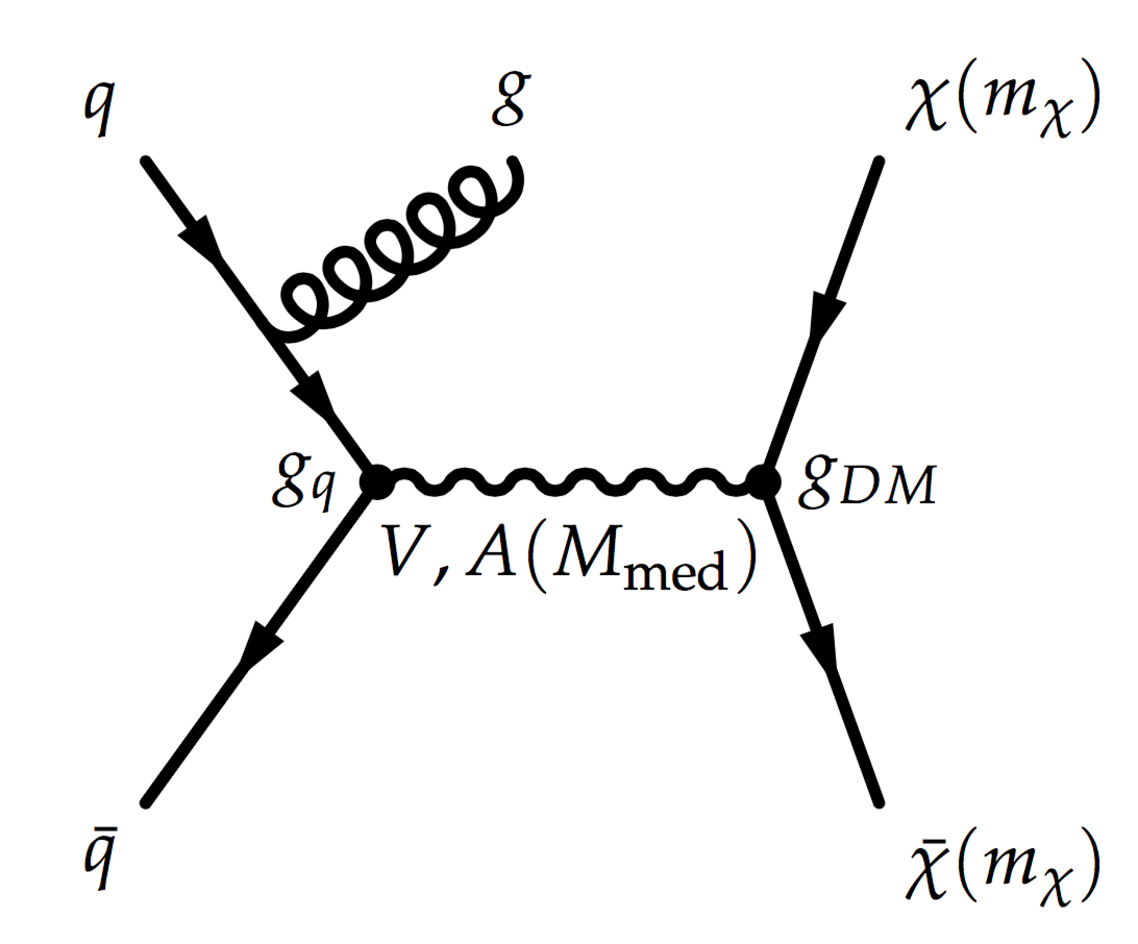
\includegraphics[width=0.35\textwidth]{figures/DMplots/feynman_light_jet.pdf}}
  \caption{Feynman diagram of DM pair production in light jet hadronic final states. \cite{Abercrombie:2015wmb}}
  \label{fig:DMfeynman} 
\end{figure}


\begin{figure}[h!] \centering
\subfigure{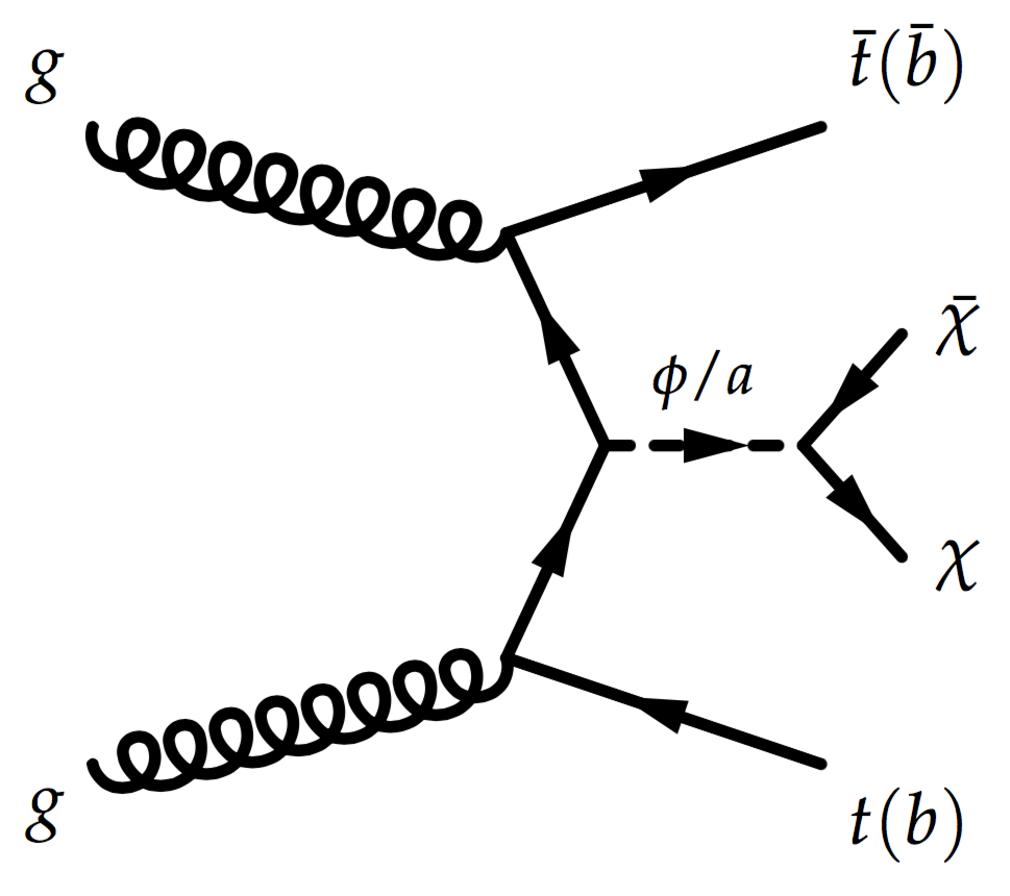
\includegraphics[width=0.35\textwidth]{figures/DMplots/feynman_hf.pdf}}
\caption{Feynman diagram of the pair production of Dark Matter particles in
association with $t\bar{t}$ or $b\bar{b}$. \cite{Abercrombie:2015wmb}}
\label{fig:feynman_hf} \end{figure}


%Assuming 2~\ifb of data we list the cross sections, yields and selection  efficiencies for the four light jet models in Tables~\ref{summaryTableAN_DMV_xs10_g0p25_2p1fb_exp}-\ref{summaryTableAN_DMS_xs10_g1p0_2p1fb_exp}. 
The signal selection efficiencies are around $\sim 1$\% for mass points near the expected exclusion
region, and are correspondingly larger (smaller) for higher (lower) mass points.
The asymmetric and monojet categories are seen to almost double the acceptance
to these models compared to the Run~1 symmetric categories alone, justifying the
inclusion of these selections into the analysis.


\begin{table}[]
\centering
\begin{tabular}{ll}
\hline \hline
Sample & NGen \\ \hline
DM+bbar PS  Mchi=1 Mmed=10  & 50246 \\
DM+bbar PS  Mchi=1 Mmed=20  & 50259 \\
DM+bbar PS  Mchi=1 Mmed=50  & 50068 \\
DM+bbar PS  Mchi=1 Mmed=200 &  50667 \\
DM+bbar PS  Mchi=1 Mmed=300 &  50905 \\
DM+bbar PS  Mchi=1 Mmed=1000 &  50680 \\
DM+bbar PS  Mchi=10 Mmed=10  & 50046 \\
DM+bbar PS  Mchi=10 Mmed=50  & 49875 \\
DM+bbar PS  Mchi=50 Mmed=10  & 50456 \\
DM+bbar PS  Mchi=50 Mmed=95  & 50205 \\
DM+bbar PS  Mchi=50 Mmed=200 &  47846 \\
DM+bbar PS  Mchi=150 Mmed=500 & 107788 \\
DM+bbar PS  Mchi=500 Mmed=10  & 51464 \\
DM+bbar PS  Mchi=500 Mmed=500 &  50283 \\
DM+bbar PS  Mchi=500 Mmed=995 &  50437 \\
DM+bbar PS  Mchi=500 Mmed=10000 &  50239 \\
DM+bbar PS  Mchi=1000 Mmed=10  & 50036 \\
DM+bbar PS  Mchi=1000 Mmed=1000 &  50960 \\
\hline \hline
\end{tabular}
\caption{DM+$b\bar{b}$ signal simulations using pseudoscalar couplings. The last number gives the number of events generated}
\label{tab:dmbb_ps}
\end{table}


\begin{table}[]
\centering
\begin{tabular}{llll}
\hline\hline
Sample & Mchi    & Mmed    & NGen \\
DM+bbar S & Mchi=1    & Mmed=10    & 47880 \\
DM+bbar S & Mchi=1    & Mmed=20    & 50036 \\
DM+bbar S & Mchi=1    & Mmed=200   & 50454 \\
DM+bbar S & Mchi=1    & Mmed=500   & 50001 \\
DM+bbar S & Mchi=1    & Mmed=1000  & 50768 \\
DM+bbar S & Mchi=1    & Mmed=10000 & 50379 \\
DM+bbar S & Mchi=10   & Mmed=10    & 49767 \\
DM+bbar S & Mchi=10   & Mmed=15    & 50377 \\
DM+bbar S & Mchi=10   & Mmed=50    & 50116 \\
DM+bbar S & Mchi=10   & Mmed=10000 & 50545 \\
DM+bbar S & Mchi=150  & Mmed=295   & 49927 \\
DM+bbar S & Mchi=150  & Mmed=10000 & 50219 \\
DM+bbar S & Mchi=500  & Mmed=10    & 50089 \\
DM+bbar S & Mchi=500  & Mmed=995   & 50040 \\
DM+bbar S & Mchi=500  & Mmed=10000 & 50206 \\
DM+bbar S & Mchi=1000 & Mmed=10    & 50576 \\
DM+bbar S & Mchi=1000 & Mmed=1000  & 50412\\
\hline \hline
\end{tabular}
\caption{DM+$b\bar{b}$ signal simulations using scalar couplings. The last number gives the number of events generated}
\label{tab:dmbb_s}
\end{table}




\begin{table}[]
\centering
\begin{tabular}{llll}
\hline \hline
Sample & $m_\chi$    & $m_\textrm{Med}$    & NGen \\ \hline  
DM+jets PS & 10  & 1      & 298400 \\
DM+jets PS & 10  & 10     & 300000 \\
DM+jets PS & 10  & 50     & 300000 \\
DM+jets PS & 10  & 100    & 297600 \\
DM+jets PS & 10  & 150    & 297400 \\
DM+jets PS & 10  & 1000   & 292800 \\
DM+jets PS & 20  & 1      & 299600 \\
DM+jets PS & 20  & 10     & 300000 \\
DM+jets PS & 50  & 1      & 298400 \\
DM+jets PS & 50  & 10     & 300000 \\
DM+jets PS & 50  & 50     & 300000 \\
DM+jets PS & 100 & 1      & 298400 \\
DM+jets PS & 100 & 10     & 300000 \\
DM+jets PS & 100 & 50     & 300000 \\
DM+jets PS & 100 & 100    & 297800\\
\hline \hline
\end{tabular}
\caption{DM+jets signal simulations using pseudoscalar couplings. The last number gives the number of events generated}
\label{tab:dmj_ps}
\end{table}


\begin{table}[]
\centering
\begin{tabular}{llll}
\hline \hline
Sample & $m_\chi$    & $m_\textrm{Med}$    & NGen \\ \hline
DM+jets  AV & 10   & 1    &300000 \\
DM+jets  AV & 10   & 10   &300000 \\
DM+jets  AV & 10   & 50   &293600 \\
DM+jets  AV & 10   & 100  &300000 \\
DM+jets  AV & 10   & 200  &300000 \\
DM+jets  AV & 10   & 250  &298400 \\
DM+jets  AV & 10   & 300  &300000 \\
DM+jets  AV & 10   & 350  &295200 \\
DM+jets  AV & 10   & 400  &288200 \\
DM+jets  AV & 20   & 1    &300000 \\
DM+jets  AV & 20   & 10   &300000 \\
DM+jets  AV & 50   & 1    &300000 \\
DM+jets  AV & 50   & 10   &291600 \\
DM+jets  AV & 50   & 50   &297400 \\
DM+jets  AV & 100  & 10   &299000 \\
DM+jets  AV & 100  & 50   &297800 \\
DM+jets  AV & 100  & 100  &297200 \\
DM+jets  AV & 200  & 50   &297400 \\
DM+jets  AV & 200  & 100  &300000 \\
DM+jets  AV & 200  & 150  &300000 \\
DM+jets  AV & 300  & 50   &288200 \\
DM+jets  AV & 300  & 100  &300000 \\
DM+jets  AV & 300  & 200  &296723 \\
DM+jets  AV & 300  & 250  &300000 \\
DM+jets  AV & 500  & 50   &295600 \\
DM+jets  AV & 500  & 100  &300000 \\
DM+jets  AV & 500  & 150  &293400 \\
DM+jets  AV & 500  & 200  &300000 \\
DM+jets  AV & 500  & 250  &300000 \\
DM+jets  AV & 500  & 300  &297000 \\
DM+jets  AV & 500  & 350  &300000 \\
DM+jets  AV & 500  & 400  &297800 \\
DM+jets  AV & 750  & 100  &295800 \\
DM+jets  AV & 750  & 250  &290800 \\
DM+jets  AV & 750  & 300  &300000 \\
DM+jets  AV & 750  & 350  &300000 \\
DM+jets  AV & 750  & 400  &296800 \\
DM+jets  AV & 1000 & 50   &298400 \\
DM+jets  AV & 1000 & 250  &286980 \\
DM+jets  AV & 1000 & 300  &300000 \\
DM+jets  AV & 1000 & 350  &298800 \\
DM+jets  AV & 1000 & 400  &296800 \\
DM+jets  AV & 1250 & 50   &300000 \\
DM+jets  AV & 1250 & 100  &297800 \\
DM+jets  AV & 1250 & 150  &298000 \\
DM+jets  AV & 1250 & 200  &296400 \\
DM+jets  AV & 1250 & 250  &296800 \\
DM+jets  AV & 1250 & 350  &272400 \\
DM+jets  AV & 1250 & 500  &285496 \\
DM+jets  AV & 1250 & 1000 &300000 \\
DM+jets  AV & 1500 & 1    &298400 \\
DM+jets  AV & 1500 & 10   &297200 \\
DM+jets  AV & 1500 & 50   &300000 \\
DM+jets  AV & 1500 & 100  &294600 \\
DM+jets  AV & 1500 & 200  &300000\\
\hline \hline
\end{tabular}
\caption{DM+jets signal simulations using axial-vector couplings. The last number gives the number of events generated}
\label{tab:dmj_av}
\end{table}


\begin{table}[]
\centering
\begin{tabular}{llll}
\hline \hline
Sample & Mchi    & Mmed    & NGen \\ \hline
DM+ttbar  PS & Mchi=1    & Mmed=10    & 252054 \\
DM+ttbar  PS & Mchi=1    & Mmed=20    & 247516 \\
DM+ttbar  PS & Mchi=1    & Mmed=50    & 255516 \\
DM+ttbar  PS & Mchi=1    & Mmed=100   & 249971 \\
DM+ttbar  PS & Mchi=1    & Mmed=200   & 240536 \\
DM+ttbar  PS & Mchi=1    & Mmed=300   & 250250 \\
DM+ttbar  PS & Mchi=1    & Mmed=500   & 244681 \\
DM+ttbar  PS & Mchi=1    & Mmed=1000  & 408173 \\
DM+ttbar  PS & Mchi=1    & Mmed=10000 & 204186 \\
DM+ttbar  PS & Mchi=10   & Mmed=10    & 249863 \\
DM+ttbar  PS & Mchi=10   & Mmed=15    & 253099 \\
DM+ttbar  PS & Mchi=10   & Mmed=50    & 252215 \\
DM+ttbar  PS & Mchi=10   & Mmed=100   & 246115 \\
DM+ttbar  PS & Mchi=10   & Mmed=10000 & 411495 \\
DM+ttbar  PS & Mchi=50   & Mmed=10    & 274874 \\
DM+ttbar  PS & Mchi=50   & Mmed=50    & 253334 \\
DM+ttbar  PS & Mchi=50   & Mmed=95    & 379662 \\
DM+ttbar  PS & Mchi=50   & Mmed=200   & 239809 \\
DM+ttbar  PS & Mchi=50   & Mmed=300   & 256765 \\
DM+ttbar  PS & Mchi=50   & Mmed=10000 & 447898 \\
DM+ttbar  PS & Mchi=150  & Mmed=10    & 293811 \\
DM+ttbar  PS & Mchi=150  & Mmed=200   & 243139 \\
DM+ttbar  PS & Mchi=150  & Mmed=295   & 278441 \\
DM+ttbar  PS & Mchi=150  & Mmed=500   & 251043 \\
DM+ttbar  PS & Mchi=150  & Mmed=1000  & 250827 \\
DM+ttbar  PS & Mchi=150  & Mmed=10000 & 374575 \\
DM+ttbar  PS & Mchi=500  & Mmed=10    & 243491 \\
DM+ttbar  PS & Mchi=500  & Mmed=500   & 258498 \\
DM+ttbar  PS & Mchi=500  & Mmed=995   & 281855 \\
DM+ttbar  PS & Mchi=500  & Mmed=10000 & 396617 \\
DM+ttbar  PS & Mchi=1000 & Mmed=10    & 240502 \\
DM+ttbar  PS & Mchi=1000 & Mmed=1000  & 440564 \\
DM+ttbar  PS & Mchi=1000 & Mmed=10000 & 317907 \\
\hline \hline
\end{tabular}
\caption{DM+$t\bar{t}$ signal simulations using pseudo-scalar couplings. The last number gives the number of events generated}
\label{tab:dmtt_ps}
\end{table}



\begin{table}[]
\centering
\begin{tabular}{llll}
\hline \hline
Sample & $m_\chi$    & $m_\textrm{Med}$    & NGen \\ \hline
DM+ttbar  S  & 1    & 10    & 240379 \\
DM+ttbar  S  & 1    & 20    & 251225 \\
DM+ttbar  S  & 1    & 50    & 253308 \\
DM+ttbar  S  & 1    & 100   & 257761 \\
DM+ttbar  S  & 1    & 200   & 254295 \\
DM+ttbar  S  & 1    & 300   & 254030 \\
DM+ttbar  S  & 1    & 500   & 250524 \\
DM+ttbar  S  & 1    & 1000  & 258859 \\
DM+ttbar  S  & 1    & 10000 & 249959 \\
DM+ttbar  S  & 10   & 10    & 245622 \\
DM+ttbar  S  & 10   & 15    & 239050 \\
DM+ttbar  S  & 10   & 50    & 254833 \\
DM+ttbar  S  & 10   & 100   & 244948 \\
DM+ttbar  S  & 10   & 10000 & 442394 \\
DM+ttbar  S  & 50   & 10    & 333199 \\
DM+ttbar  S  & 50   & 50    & 245362 \\
DM+ttbar  S  & 50   & 95    & 242838 \\
DM+ttbar  S  & 50   & 200   & 251025 \\
DM+ttbar  S  & 50   & 300   & 252187 \\
DM+ttbar  S  & 50   & 10000 & 495036 \\
DM+ttbar  S  & 150  & 10    & 535684 \\
DM+ttbar  S  & 150  & 200   & 237784 \\
DM+ttbar  S  & 150  & 295   & 383362 \\
DM+ttbar  S  & 150  & 500   & 219636 \\
DM+ttbar  S  & 150  & 1000  & 222381 \\
DM+ttbar  S  & 150  & 10000 & 366184 \\
DM+ttbar  S  & 500  & 10    & 242850 \\
DM+ttbar  S  & 500  & 500   & 253947 \\
DM+ttbar  S  & 500  & 995   & 257082 \\
DM+ttbar  S  & 500  & 10000 & 382104 \\
DM+ttbar  S  & 1000 & 10    & 435870 \\
DM+ttbar  S  & 1000 & 1000  & 362123 \\
DM+ttbar  S  & 1000 & 10000 & 317556 \\
\hline \hline
\end{tabular}
\caption{DM+$t\bar{t}$ signal simulations using scalar couplings. The last number gives the number of events generated}
\label{tab:dmtt_s}
\end{table}




%Currently we are scaling the expected sensitivities to 2.2~\ifb of data corresponding to last years dataset to be able to compare.
%The expected 95\% CL signal strength for vector-axial (VA) samples with couplings to the SM of $g_\textrm{SM}=0.25$ and $g_\textrm{DM}=0.25$
%is showin on Fig.~\ref{fig:exp_dmj_av}



%\begin{figure}[h!] \centering
%\subfigure{\includegraphics[width=0.35\textwidth]{figures/DMplots/DMA_76X_ContourLimits.pdf}}
%\caption{Expected sensitivities for 2.2~\ifb for the Axial-Vector light jet DM models}
%\label{fig:exp_dmj_av} \end{figure}




%Owing to the principal of Minimal Flavor Violation (MFV), top and bottom quarks can play important roles in the phenomenology of dark matter. Scalar and
%pseudoscalar models predict not only the `monojet' processes described in Sec.~\ref{sec:dm_lightjet} but also the production of dark matter in association
%with top (or bottom) pairs. This results in signatures with relatively large jet multiplicities, in particular for \DMtt production. The \alphat analysis is well 
%suited to searching for such signatures. An example Feynman diagram for the pair production of dark matter particles in association with pairs of heavy quarks is
%shown in Fig.~\ref{fig:feynman_hf}.



%\begin{figure}[h!] \centering
%\subfigure{\includegraphics[width=0.35\textwidth]{figures/DMplots/DMA_76X_ContourLimits.pdf}}
%\caption{Expected sensitivities for 2.2~\ifb for the pseudo-scalar DM+$t\bar{t}$ models}
%\label{fig:exp_dmtt_ps} \end{figure}


%Finally we show the sensitivity jet rakings in Fig....



